% !TeX root = ../main.tex

\chapter{相关工作}
\label{cha:related_work}

知识图谱应用广泛,在众多下游任务中发挥着不可替代的作用,例如信息检索、知识问答、文本生成等。然而知识图谱的构建是一个非常耗费时间、耗费人力物力的工作。因此,关系抽取任务便应运而生。关系抽取任务旨在给定文本及文本中两个实体后,推理出两个实体之间的关系。关系抽取任务是知识图谱构建自动化的关键,该任务要求模型能够阅读文本并理解文本。自该任务提出以来,便受到学者的广泛关注。本章节将从句子级别关系抽取和文档级别关系抽取两个角度介绍已有的关系抽取的工作,同时本文还将介绍预训练模型的相关工作。本工作希望能够利用预训练的形式,充分利用文档级别远程监督数据,提升模型对于文档的理解能力并在文档级关系抽取任务上取得更好的效果。

\section{句子级别关系抽取}

现有的大多数关系抽取工作,都聚焦于句子级别关系抽取,即从一个句子中抽取出给定两个实体的关系。这些工作大致可以分成以下几类。
%早期的工作主要关注于使用统计机器学习算法来从句子中获取句法特征从而预测出句子中包含的关系类型。

%\subsection{传统模型}
\subsection{模式抽取模型} 
早期有许多工作聚焦于用句法分析工具来抽取出句子中的句法元素、属性,并根据这些元素与属性自动构建出表达了某种关系语义的句式规则,以此达到抽取关系的目的\cite{soderland1995crystal,kim1995acquisition,mooney1999relational}。随后为了让自动构建的句式具有足够的精确性及召回率,之后的许多工作尝试使用更大的语料库\cite{carlson2010toward},以及更多类型的句式\cite{nakashole2012patty,jiang2017metapad}。但是语言的表达的多样性给这样一种方式带来了天然的限制,任何一种算法都无法穷举完所有的表达方式,因此基于模式抽取的关系抽取模型在召回率方面表现相对较差。

\subsection{基于统计学习算法的抽取模型}
基于统计学习算法的模型中有很重要的一类是基于特征工程的抽取模型。这一类模型通过设计词法、句法、语义特征,并将这些特征喂入关系分类器中达到关系抽取的目的\cite{kambhatla2004combining,guodong2005exploring,jiang2007systematic}。同时,由于支持向量机(Support Vector Machine,SVM)的有效性在许多分类任务上得到了证明,不少基于核方法的关系抽取模型被相继提出\cite{culotta2004dependency,bunescu2005shortest,zhang2006composite}。这些算法通过设计多种多样的核函数,来计算关系表示及句子表示之间的相似度。同时,也有许多工作关注于如何更好的利用句子中句法依赖关系,从而提出基于图的模型\cite{roth2002probabilistic,sarawagi2005semi,yu2010jointly}。图能够很好地将句子中实体、词语等元素之间的依赖关系抽象成有向无环图,并利用这种结构信息来挖掘句子的语义信息。同样的,基于统计学习算法的抽取模型依旧面临着很大的挑战。基于特征工程的抽取模型和基于核方法的抽取模型都需要针对于语料库和不同的关系类型设计不同的特征以及核函数,可扩展性较差。图模型可以在没有很多人工干预的情况下抽取出不同的关系,但模型在准确率上表现依旧有限。

%\subsection{神经网络模型}

\subsection{神经网络关系抽取}
\begin{figure*}
	\centering
	\includegraphics[width = \textwidth]{related_work/supervised_re.pdf}
	\caption{神经网络关系抽取模型框架}
	\label{fig:related_work:supervised_re}
\end{figure*}

随着深度学习技术的发展,有许多利用端到端深度神经网络的工作在句子级别关系抽取任务上取得了很大的成功。相比于传统的基于统计学习算法的模型而言,神经网络模型可以自动抽取出文本特征,在效果上及可扩展性上都有了大幅提升。基于神经网络的抽取模型重点在于设计网络架构来更好地抽取出文本特征。许多学者尝试使用卷积神经网络(Convolutional Neural Network, CNN)来更好地对文本的局部句法特征进行建模\cite{liu2013convolution,zeng2014relation,nguyen2015relation}。也有许多工作\cite{zhang2015bidirectional,vu2016combining}提出使用循环神经网络(Recurrent Neural Network,RNN)对文本建模,从而实现更好的长序列处理,取得更好的效果。也有许多学者相继提出多种不同的注意力机制,来帮助模型更好地利用文本中全局的关系信息\cite{zhou2016attention,wang2016relation,xiao2016semantic}。基于统计学习算法的抽取模型将人工设计的特征作为输入,再根据特征利用分类算法对文本及其中的实体对进行分类。而神经网络关系抽取模型往往将词向量和位置向量作为输入,利用神经网络作为编码器获得句子表示,再利用全连接层将句子表示映射成关系分数,如图\ref{fig:related_work:supervised_re}所示。词向量在许多NLP任务中被广泛应用,词向量利用大量无监督语料进行预训练,将词语的语义映射到连续的向量空间当中。有许多具有影响力的词向量模型被相继提出,例如Word2vec\cite{mikolov2013distributed},Glove\cite{pennington2014glove},ELMO\cite{peters2018deep}等。为了能够区分开句子中的实体和普通单词,Zeng et al.\cite{zeng2014relation}提出使用位置向量对文本中的头尾实体进行标记。

除了利用词向量信息和位置向量信息以外,也有许多工作尝试在神经网络中利用句法信息来帮助模型进行更好的预测。Xu et al.\cite{xu2015classifying}利用头实体和尾实体在句法分析树上最短的路径来捕捉句子中表达二者关系的关键信息。Liu et al.\cite{liu2015dependency}提出增强依赖路径来进一步对句法分析树上最短路径的关键信息进行建模。


\subsection{远程监督关系抽取}
\begin{figure*}
	\centering
	\includegraphics[width = \textwidth]{related_work/distant_re.pdf}
	\caption{远程监督关系抽取示例\cite{yao2019docred}。根据关系事实(\texttt{Apple Inc.}, \textit{product}, \texttt{iPhone}),远程监督机制找到所有带有实体\texttt{Apple Inc.}和\texttt{iPhone}的句子,并将它们标注成关系\textit{product}。远程监督机制可以有效扩充数据集,但也不可避免地带来许多噪音。}
	\label{fig:related_work:distant_re}
\end{figure*}

上述基于深度学习的模型在很多关系抽取数据集上的效果取得了很大的提升。但是以上方法都非常依赖于大规模的高质量的手工标注数据集,而这样的数据集的构建是需要有非常大的人力物力消耗及时间消耗的。为了解决这个问题,远程监督机制\cite{mintz2009distant,nguyen2011end,min2013distant}被提出。远程监督机制可以自动标注数据,构建大规模的关系抽取数据集。该机制假设:给定一个知识图谱中的关系事实$(h, r, t)$,那么任何一个包含有实体$h$和实体$t$的句子都将表述这两个实体的关系。因此,包含有实体对$(h, r)$的句子都将被自动标注为关系$r$。正如图\ref{fig:related_work:distant_re}所示,给定关系事实(\texttt{Lebron James}, \textit{member\_of}, \texttt{Lakers}),远程监督机制将在大规模的语料库中寻找包含实体\texttt{Lebron James}和实体\texttt{Lakers}的句子,并将这些句子及其中包含的实体对标注成关系$r$。按照这样的规则,可以很简单地构造出非常大规模的数据集。

因此,远程监督机制可以使得模型能够利用更多的数据进行训练。然而这样一种自动标注的机制也将给数据集带来较多的错误标注的问题。并不是任何一个包含有实体对$(h,r)$的句子,都能够表述出这两个实体之间的关系。正如图\ref{fig:related_work:distant_re}中第三个句子所示,\texttt{Lebron James said he wants to be in the Lakers for the rest of his life.}即使句子中包含\texttt{Lebron James}和\texttt{Lakers}两个实体,但是这个句子并没有阐述二者之间的关系。因此,远程监督机制带来数据量大幅增加的好处的同时,也给关系抽取模型提出了新的挑战:如何应对数据集中的噪音。为了解决这个问题,许多学者做出了有益探索,这些工作大体可以分成以下三类:
\begin{itemize}
	\item 利用多示例学习(multi-instance learning)的框架进行建模,将包含有相同实体对的句子组合成一个包,模型需要从每个包中挑选出有可能阐述两个实体关系的句子。Zeng et al.\cite{zeng2015distant}提出一个非常简单的启发式策略,从每个包中挑选出置信度最高的样例来更新模型参数。然而往往一个包中不止有一个样例为正确标注样例,因此有许多学者设计了很多不同的注意力机制,为包中每个不同的样例赋予不同的权重,进而通过对样例的表示进行加权平均得到给定实体对的关系表示,以此实现充分利用数据的同时筛除错误标注的噪音\cite{lin2016neural,han2018hierarchical,zhu2019improving}。
	\item 利用文本以外的信息进行样例挑选,例如利用实体描述\cite{ji2017distant}和知识图谱\cite{han2018neural,qu2019fine}作为额外信息,帮助判断句子是否为噪音数据。同时也有学者探索使用多语言的语料库来保证信息的一致性和互补性\cite{verga2016multilingual,lin2017neural,wang2018adversarial}。
	\item 利用更鲁棒的机制和训练策略。Vu et al.\cite{vu2016combining}结合了循环神经网络和卷积神经网络两种结构来得到更鲁棒的网络结构。Liu et al.\cite{liu2017soft}引入了软标签机制,在训练过程中修改置信度低的样例的标签。随后,利用强化学习\cite{feng2018reinforcement,zeng2018large}和对抗学习\cite{wu2017adversarial,wang2018adversarial}进行降噪的训练策略也被不断应用于远程监督关系抽取任务。
\end{itemize}

远程监督机制给耗时耗力的关系标注提供了解决措施,但同时也不可避免地引入了错误标注的噪音。如何实现更好的远程监督机制和对噪音更加包容的训练模式依旧是一个很大的挑战。

%\subsection{多实体关系推理} 

\section{文档级别关系抽取}
\begin{figure*}
	\centering
	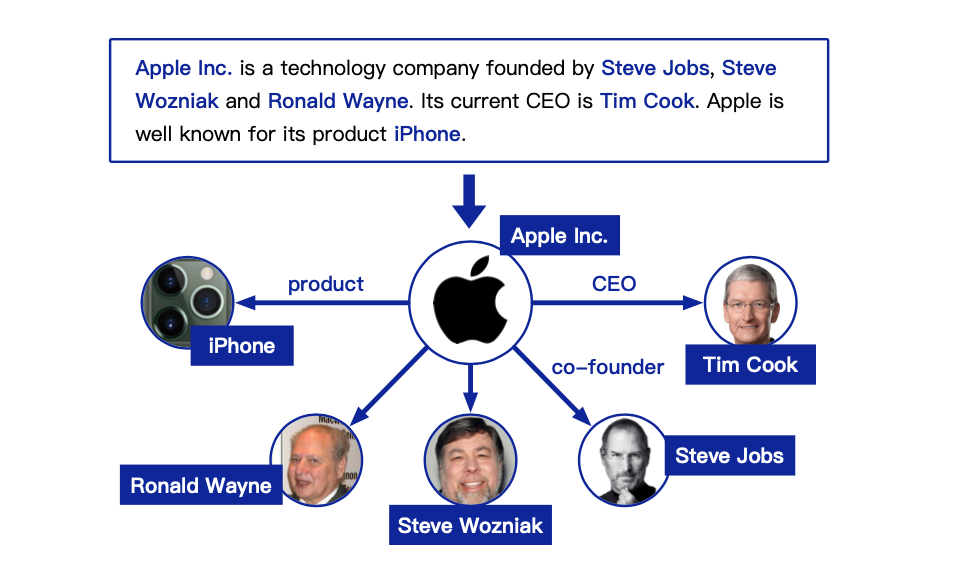
\includegraphics[width = 0.8\textwidth]{related_work/doc_re.png}
	\caption{一个文档级关系抽取的样例。给定一个包含有多个句子、多个实体的文档,模型需要抽取出文档中包含的所有关系事实。}
	\label{fig:related_work:doc_re}
\end{figure*}

目前大部分关系抽取的工作都是针对于句内关系的抽取,而忽略了文档级别句间关系的抽取。有许多关系事实往往涉及复杂的关系推理,用一句话难以表述清楚。在这样的情况下,句子级别关系抽取就无法有效地抽取出关系事实。据数据显示,在一篇文档中有$40.7\%$的关系事实必须通过多实体、跨句推理才能够抽取得到\cite{yao2019docred}。因此,将关系抽取任务从句子级别扩展到文档级别是非常必要的。

与句子级别关系抽取不同,一个文档中往往包含有非常多的实体,实体与实体之间也有着丰富多样的关系类型。同时,文档级别关系抽取任务的定义也与句子级别关系抽取定义有着一些不同。如图\ref{fig:related_work:doc_re}所示,文档级关系抽取旨在给定一篇文档及其中包含的实体时,抽取出这些实体之间所有的关系事实。在本小节,我将介绍主要文档级别关系抽取的数据集和现有的一些工作。

\subsection{文档级别关系抽取数据集}
从事文档级关系抽取的研究便要求有大规模的文档级别关系抽取的数据集,用来进行模型的训练及测试。随着文档级关系抽取受到越来越多的关注,也有学者相继提出了一些文档级别关系抽取的数据集。
Quirk et al.\cite{quirk2017distant}从PubMed\footnote{http://www.ncbi.nlm.nih.gov/pmc/}上获取了大量的无标注的生物医学文献,并将文档中的药物及基因实体识别出来,并与基因药物知识库(Gene Drug Knowledge Database,GDKD)中实体对齐,将在三句之内的关系,利用远程监督机制标注出来。Peng et al.\cite{peng2017cross}与前者类似,利用同样的机制从大量的无标注的生物医学文献中标注关系,但该工作主要关注于基因、药物、突变三者的多元关系。前面两个数据集关注到跨句关系推理,但都将数据语料限制在三句之内,无法真正做到文档级别关系抽取。并且这两个数据集没有进行人工标注,而使用带有噪音的远程监督数据来测试模型,这也导致了测试结果相对来说具有比较大的不可靠性。Li et al.\cite{li2016biocreative}提出了一个包含有$1,500$篇PubMed文档的手工标注数据集,该数据集专注于生物医学领域的“化学性疾病”这一关系。Yao et al.\cite{yao2019docred}提出DocRED数据集,该数据集基于维基百科进行构建,人工标注 $5,053$ 篇文档中包含的实体和关系。各个数据集具体的数据对比见\ref{table:related_work:dataset_stat}。

\begin{table}[]
\centering
\begin{tabular}{lrrrrrrr}
\toprule
Dataset             & \# Doc. & \# Word & \# Sent. & \# Ent.   & \# Rel. & \# Inst.  & \# Fact \\
\midrule
SemEval-2010 & -       & 205k    & 10,717   & 21,434    & 9       & 8,853     & 8,383   \\
ACE 2003-2004       & -       & 297k    & 12,783   & 46,108    & 24      & 16,771    & 16,536  \\
TACRED              & -       & 1,823k  & 53,791   & 152,527   & 41      & 21,773    & 5,976   \\
FewRel              & -       & 1,397k  & 56,109   & 72,124    & 100     & 70,000    & 55,803  \\
\midrule
BC5CDR              & 1,500,  & 282k    & 11,089   & 29,271    & 1       & 3,116     & 2,434   \\
DocRED\_a   & 50,053  & 1,002k  & 40,276   & 132,375   & 96      & 63,427    & 56,354  \\
DocRED\_d      & 101,873 & 21,368k & 828,115  & 2,558,350 & 96      & 1,508,320 & 881,298 \\
\bottomrule
\end{tabular}
\caption{各个关系抽取数据集的详细数据展示。其中Doc指文档数,Word指总共单词数量,Sent指句子数量,Ent指实体数量,Rel指关系数量,Inst指关系实例数量,Fact指关系事实数量。DocRED\_a指DocRED中人工标注数据集,DocRED\_d指DocRED中远程监督数据集。}
\label{table:related_work:dataset_stat}
\end{table}


\subsection{跨句关系抽取}
早期有很多工作关注于从跨句的关系抽取。许多学者\cite{swampillai2011extracting,yoshikawa2011coreference,quirk2017distant}聚焦于抽取出多个句子中的句法特征,利用句法特征将不同的句子连接在一起,再利用统计学习算法将特征分类到不同的关系中。常用的句法特征包括:实体指代特征、最短路径树、语法依存关系等。也有许多学者\cite{zeng2017incorporating,christopoulou2018walk}将不同的句子中的实体按照句内关系构成一个图,通过头尾实体之间的多跳路径来推理出实体之间的关系。\citet{peng2017cross,song2018n}则利用图神经网络(Graph Neural Network,GNN)来进行多实体、跨句的推理,图神经网络的运用给模型记忆能力、推理能力都带来了较大的提升。


\subsection{文档级关系抽取}
文档级关系抽取比之前工作提到的跨句关系抽取更加复杂,文档中多个句子具有较强的关联,且实体数量也要多很多。\citet{nguyen2018convolutional,li2018chemical}关注于生物医学、化学等特定领域的文档级关系抽取,并将之前句子级别关系抽取的模型直接利用至文档级别。但是由于传统模型,例如CNN、RNN等,在处理长的文本序列时,将遇到灾难性遗忘问题,因此模型无法充分利用实体的上下文信息。因此,有许多学者关注到使用图结构对篇章级别的文本进行建模,旨在建立起文档中长距离的、跨句子的信息流动,从而更好的实现多实体间的多步推理。\citet{quirk2017distant}构造了句内的依存边和句间的依存边来连接不同的实体。\citet{sahu2019inter}将词语作为结点,提出了五种边的类型:句法依存关系边、指代边、相邻句子边、相邻词语边、自环边,构造了一个文档级别的图结构,并利用图卷积神经网络(Graph Convolutional Neural Network)来学习结点表示,并将结点表示直接运用到最后关系分类中。而与此相反,\citet{christopoulou2019connecting}按照类似的方式构建了文档级的图结构,但其关注于边的表示的学习,并提出了一种以边为核心的图神经网络,将边的表示作为关系表示,运用于关系分类器中。

与之前的工作不同,本文提出的模型注重于通过预训练的模式高效地利用噪音很大的远程文档级监督数据。据我所知,本文是第一个在文档级别关系抽取中使用预训练的方式利用远程监督数据的工作。



\section{预训练模型}
\subsection{预训练语言模型}
预训练作为迁移学习的经典范式之一,在自然语言处理领域、计算机视觉领域都被广泛应用。计算机视觉领域许多研究也相继证明了基于预训练模型的迁移学习是十分有效的\cite{deng2009imagenet,yosinski2014transferable}。同样,在自然语言处理领域,预训练语言模型也得到了广泛的研究和应用。这些工作可以分成基于特征的预训练语言模型和基于微调的预训练语言模型两类。基于特征的预训练语言模型的工作\cite{mikolov2013distributed,pennington2014glove,peters2018deep}注重于将每一个词语映射到一个低维度、稠密的向量空间中,并将词语向量作为特征运用到下游的自然语言处理的相关任务当中。这些通过预训练得到的单词表示包含了丰富的句法特征和词意特征,所以这些向量经常被当做各种模型的输入,相比于利用随机初始化的词向量作为输入,这种方法在效果上取得了很大的提升。与基于特征的预训练语言模型仅运用预训练过程得到的词向量作为输入特征不同,基于微调的预训练语言模型将模型结构、参数都保留,作为下游任务模型训练的起点\cite{dai2015semi,howard2018universal,merity2017regularizing,devlin2019bert}。
其中\citet{devlin2019bert}提出的双向深度Transformer模型(Bert)取得了多个自然语言处理任务的最佳效果,因此该模型被广泛应用。本文的工作也是基于Bert模型开展实验。

\subsection{预训练关系表示学习}
随着预训练语言模型在很多任务上被证明是非常有效的,有许多学者\cite{du2018multi,wu2019enriching}也探索了如何将预训练语言模型运用到关系抽取任务上,这也在很多数据集上实现了最佳效果。也有许多学者聚焦于如何让模型学习可迁移的关系表示。\citet{wu2019open}提出了关系孪生网络,在有监督的数据集上让相同的关系有相似的表示,并将模型迁移至无监督数据上,实现了关系知识的迁移。进一步地,\citet{soares2019matching}提出,在大规模远程监督的句子级别关系抽取数据集上,学习有效的关系表示。与之前工作类似,该文章通过让出现在不同句子的相同的关系事实表示相近,让不同的关系事实表示距离变远来训练一个关系表示编码器。实验证明,该模型在关系抽取的有监督场景和少样本学习场景中效果均有明显提升。

然而,在文档级别远程监督数据中,噪音比例要远大于句子级别远程监督数据。因此,上述训练过程会因噪音过多而无法收敛。本文聚焦于在文档级别远程监督数据上进行模型预训练,通过提出的三种预训练任务充分学习关系表示。









